\newcommand{\qcOne}{\mathbf{1}}   %
\newcommand{\qcTwo}{\mathbf{2}}   %
\newcommand{\qcThree}{\mathbf{3}} %
\newcommand{\qcN}{\mathbf{n}}     %
\newcommand{\qcInt}{\mathbb{I}}   %
\newcommand{\qcEquiv}{\rightsquigarrow}                 %
\newcommand{\qcTFib}{\overset{\wr}{\twoheadrightarrow}} %

\section{\trQuasiCategory}\label{sec:quasi-categories}

在引入一套公理化框架、以便一般地发展 \trInfinityCategory{}理论之前，
我们先专门考察一个模型：\textbf{\trQuasiCategory}（quasi-category）——
它由 Boardman 与 Vogt 在其\trHomotopy{}相干图（homotopy coherent diagram）研究中
于 1973 年引入\cite{bib21}。通常的 1-\trCategory{}经由\cref{def:nerve}的构造给出%
\trQuasiCategory{}的例子。Joyal 在\cite{bib61}与\cite{bib63}以及若干未出版的书稿
草稿中率先承担起把 1-\trCategory{}理论\trExtension{}为\trQuasiCategory{}理论的任务；本节的大多数结果
都归功于他。

\begin{notation}[\trSimplexCategory]\label{not:simplex-category}
记 $\Delta$ 为由有限非空序数 $[n]=\{0<1<\cdots<n\}$ 及保序映射构成的
\textbf{\trSimplexCategory}（simplex category）。其中特别包括
\[
\begin{array}{ccccc}
\text{初等\trFaceOperator} & [n-1] & \xrightarrow{\;\delta^i\;} & [n] & 0\le i\le n\\
\text{初等\trDegeneracyOperator} & [n+1] & \xrightarrow{\;\sigma^i\;} & [n] & 0\le i\le n
\end{array}
\]
其像分别在元素 $i\in[n]$ 处略去、重复该元素。$\Delta$ 中每个态射都唯一地
分解为一个\trEpimorphism{}后接一个\trMonomorphism{}；这些\trEpimorphism{}即\textbf{\trDegeneracyOperator}
（degeneracy operator），可分解为初等\trDegeneracyOperator{}的复合；而\trMonomorphism{}即
\textbf{\trFaceOperator}（face operator），可分解为初等\trFaceOperator{}的复合。
\end{notation}

\textbf{\trSimplicialSet}（simplicial set）的\trCategory{}是\trSimplexCategory{}上预层
（presheaf）的\trCategory{}，记作
$s\mathcal{S}et\coloneqq\mathcal{S}et^{\Delta^{\mathrm{op}}}$。
我们以 $\Delta[n]$ 记\textbf{标准 $n$-\trSimplex}（standard $n$-simplex），
即由 $[n]\in\Delta$ 所表示的\trSimplicialSet{}；并以
$\Lambda^k[n]\subset\partial\Delta[n]\subset\Delta[n]$ 记它的
\textbf{$k$-\trHorn}（$k$-horn）与\textbf{\trBoundarySphere}（boundary sphere）。
\yizhu{horn 直译为「角」；本译取「\trHorn」，以便「内\trHorn」「外\trHorn」
「左外\trHorn」等复合词读感统一。}球面 $\partial\Delta[n]$ 是由 $n$-\trSimplex{}余维数
为一的诸面生成的单纯子集，而\trHorn $\Lambda^k[n]$ 是再略去顶点 $k$
对面的那个面所得的单纯子集。

给定\trSimplicialSet $X$，习惯上以 $X_n$ 记它的 $n$-\trSimplex{}之集，即在 $[n]\in\Delta$
处取值所得。由\trYonedaLemma{}，每个 $n$-\trSimplex{} $x\in X_n$ 对应一个\trSimplicialSet
映射 $x\colon\Delta[n]\to X$。相应地，记 $x\cdot\delta^i$ 为该 $n$-\trSimplex{}的
第 $i$ 个面，即由复合映射
\[
\Delta[n-1]\xrightarrow{\;\delta^i\;}\Delta[n]\xrightarrow{\;x\;}X
\]
分类的 $(n-1)$-单纯形。\trFaceOperator{}的右作用定义了映射
$X_n\xrightarrow{\;\cdot\delta^i\;}X_{n-1}$。几何上，$x\cdot\delta^i$
就是 $n$-\trSimplex{} $x$ 中「顶点 $i$ 对面的面」。

\begin{definition}[\trQuasiCategory]\label{def:quasi-category}
\trQuasiCategory{}是一个\trSimplicialSet $A$，其中任何\textbf{内\trHorn}
（inner horn）都能\trExtension{}为\trSimplex{}，即求解图示的\trLifting{}问题（lifting problem）：
\begin{rveq}\label{eq:inner-horn-lifting}
\mbox{\begin{tikzpicture}[x=1.5em,y=1.5em]
  \node (tl) at (0,1.3) {$\Lambda^k[n]$};
  \node (tr) at (3.0,1.3) {$A$};
  \node (bl) at (0,0) {$\Delta[n]$};
  \draw[->] (tl) -- (tr);
  \draw[->] (0,0.95) -- (0,0.3);
  \draw (0,0.95) arc[start angle=180,end angle=0,radius=0.16];
  \draw[->,dashed] (0.45,0.2) -- (2.7,1.15);
  \node at (8.3,0.65) {对 $n\ge 2$，$0<k<n$。};
\end{tikzpicture}}
\end{rveq}
\end{definition}

\trQuasiCategory{}由 Boardman 与 Vogt 首次引入\cite{bib21}，当时称作「弱\trKanComplex」——
\textbf{\trKanComplex}（Kan complex）指沿一切\trHorn{}包含 $n\ge 1$，$0\le k\le n$
都能给出如\eqref{eq:inner-horn-lifting}那样的\trExtension{}的\trSimplicialSet{}。
由于任何拓扑空间都能编码为\trKanComplex{}，\footnote{总奇异复形（total singular
complex）构造定义了从拓扑空间到\trSimplicialSet{}的一个\trFunctor{}，它在两者的\trHomotopyCategory{}上是%
\trEquivalence{}：空间的弱\trHomotopy{}型对应\trKanComplex{}的\trHomotopy\trEquivalence{}类\cite{bib93}。由
\cref{ex:nerve-cosimplicial}构造的左\trAdjunction{}则把\trSimplicialSet{}「几何实现」为一个
拓扑空间。}空间便以此方式给出\trQuasiCategory{}的例子。

\trCategory{}也经由\trNerve{}（nerve）构造给出\trQuasiCategory{}的例子。

\begin{definition}[\trNerve]\label{def:nerve}
1-\trCategory{}的\trCategory $\mathcal{C}at$ 经由\textbf{\trNerve{}函子}（nerve functor）
\trFullyFaithful{}嵌入\trSimplicialSet{}的\trCategory{}。1-\trCategory $C$ 的\trNerve{}中的 $n$-单纯形是 $C$ 中
$n$ 个可合成箭头的序列，\trEquivalence{}地，是一个从\trOrdinalCategory{}（ordinal category）
$\qcN+\qcOne\coloneqq[n]$ 到 $C$ 的\trFunctor——该\trCategory{}有对象
$0,\ldots,n$，并且恰在 $i\le j$ 时才有唯一箭头 $i\to j$。
\end{definition}

映射 $[n]\mapsto\qcN+\qcOne$ 定义了一个\trFullyFaithful{}嵌入
$\Delta\hookrightarrow\mathcal{C}at$。从这个观点看，\trNerve{}函子可以描述为
一部「限制的\trYonedaEmbedding」：它把\trCategory{} $C$ 送到可表示\trFunctor
$\mathrm{hom}(-,C)$ 在这一包含的像上的限制。更一般的「\trNerve{}型构造」见
\cref{ex:nerve-cosimplicial}。

\begin{remark}\label{rem:nerve-2-coskeletal}
\trCategory{} $C$ 的\trNerve{}作为\trSimplicialSet{}是\textbf{\trTwoCoskeletal}（2-coskeletal），
意即每个 $n\ge 3$ 的球面 $\partial\Delta[n]\to C$ 都由 $C$ 中某个
$n$-\trSimplex{}唯一填充（见定义 C.5.2）。%
注意：球面 $\partial\Delta[2]\to C$ 能\trExtension{}成一个 2-\trSimplex{}，当且仅当沿其对角
边的箭头是内\trHorn $\Lambda^1[2]\subset\partial\Delta[2]\to C$ 中沿诸边的
那些箭头的复合。维数 3 及以上的\trSimplex{}则见证：沿其\textbf{\trSpine}（spine）——
由连接相邻顶点的边组成的 1-骨架单纯子集——的可合成箭头路径，其合成满足
结合律。事实上，正如\cref{prop:nerves-quasi-categories}的证明所提示的，
任何内\trHorn{}都有\emph{唯一}\trFiller{}的\trSimplicialSet{}都\trIsomorphism{}于某个 1-\trCategory{}的\trNerve
（见\cref{ex:unique-fillers}）。
\end{remark}

我们不愿为\trNerve{}函子引入显式记号，而更愿意把 1-\trCategory{}与它们的\trNerve{}等同起来。
我们将发现：1-\trCategory{}的理论可以这样\trExtension{}到以\trQuasiCategory{}为模型的%
\trInfinityCategory{}上，使得每个 \trInfinityCategory{}概念沿\trNerve{}嵌入的限制都恢复出
相应的 1-\trCategory{}概念。例如，标准单纯形 $\Delta[n]$ \trIsomorphism{}于\trOrdinalCategory
$\qcN+1$ 的\trNerve{}，于是我们时常采用后一种记号——写
$\qcOne\coloneqq\Delta[0]$，$\qcTwo\coloneqq\Delta[1]$，$\qcThree\coloneqq\Delta[2]$，
如此等等——以暗示正确的\trCategory{}直觉。\yizhu{原书以空心数字
$\qcOne$、$\qcTwo$、$\qcThree$ 分别记 $\Delta[0]$、$\Delta[1]$、$\Delta[2]$；
译本以粗体数字近似排印。}

要沿这条路走下去，必须先核实刚刚隐含作出的那个断言：

\begin{proposition}[\trNerve{}是\trQuasiCategory]\label{prop:nerves-quasi-categories}
\trCategory{}的\trNerve{}是\trQuasiCategory{}。
\end{proposition}
\begin{proof}
经由\cref{rem:nerve-2-coskeletal}中的\trIsomorphism $C\cong\mathrm{cosk}_2\,C$
与 C.5.2 中的\trAdjunction{} $\mathrm{sk}_2\dashv\mathrm{cosk}_2$，
下方左侧所示的\trLifting{}问题转置为右侧所示者：
\begin{center}
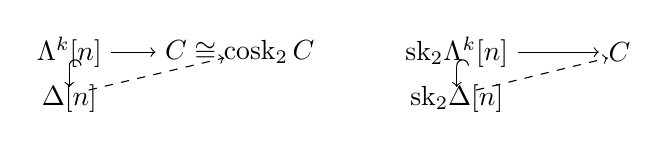
\begin{tikzpicture}[x=1.4em,y=1.4em]
  \node (tl) at (0,1.2) {$\Lambda^k[n]$};
  \node (tr) at (4.4,1.2) {$C\cong\mathrm{cosk}_2\,C$};
  \node (bl) at (0,0) {$\Delta[n]$};
  \draw[->] (tl) -- (tr);
  \draw[->] (0,0.85) -- (0,0.3);
  \draw (0,0.85) arc[start angle=180,end angle=0,radius=0.15];
  \draw[->,dashed] (0.5,0.22) -- (4.0,1.05);
  \node at (7.2,0.6) {$\leftrightsquigarrow$};
  \node (tl2) at (10.0,1.2) {$\mathrm{sk}_2\Lambda^k[n]$};
  \node (tr2) at (14.2,1.2) {$C$};
  \node (bl2) at (10.0,0) {$\mathrm{sk}_2\Delta[n]$};
  \draw[->] (tl2) -- (tr2);
  \draw[->] (10.0,0.85) -- (10.0,0.3);
  \draw (10.0,0.85) arc[start angle=180,end angle=0,radius=0.15];
  \draw[->,dashed] (10.5,0.22) -- (13.9,1.05);
\end{tikzpicture}
\end{center}
\trFunctor{} $\mathrm{sk}_2$ 把\trSimplicialSet{}替换成它的\textbf{2-\trSkeleton}
（2-skeleton）：由维数至多 2 的\trSimplex{}生成的单纯子集。
当 $n\ge 4$ 时，
包含 $\mathrm{sk}_2\Lambda^k[n]\hookrightarrow\mathrm{sk}_2\Delta[n]$
是\trIsomorphism{}，此时右侧的\trLifting{}问题有（唯一的）解。于是只剩下 $n=2$ 与 $n=3$
两种情形需要求解左侧的\trLifting{}问题。为此考察
\begin{center}
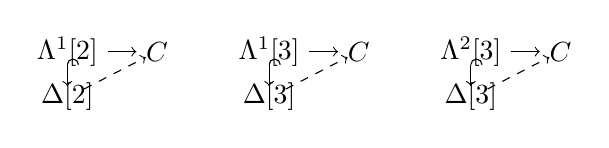
\begin{tikzpicture}[x=1.35em,y=1.35em]
  \node (a1) at (0,1.2) {$\Lambda^1[2]$};
  \node (a2) at (2.4,1.2) {$C$};
  \node (a3) at (0,0) {$\Delta[2]$};
  \draw[->] (a1) -- (a2);
  \draw[->] (0,0.85) -- (0,0.28);
  \draw (0,0.85) arc[start angle=180,end angle=0,radius=0.15];
  \draw[->,dashed] (0.45,0.2) -- (2.1,1.05);
  \node (b1) at (5.4,1.2) {$\Lambda^1[3]$};
  \node (b2) at (7.8,1.2) {$C$};
  \node (b3) at (5.4,0) {$\Delta[3]$};
  \draw[->] (b1) -- (b2);
  \draw[->] (5.4,0.85) -- (5.4,0.28);
  \draw (5.4,0.85) arc[start angle=180,end angle=0,radius=0.15];
  \draw[->,dashed] (5.85,0.2) -- (7.5,1.05);
  \node (c1) at (10.8,1.2) {$\Lambda^2[3]$};
  \node (c2) at (13.2,1.2) {$C$};
  \node (c3) at (10.8,0) {$\Delta[3]$};
  \draw[->] (c1) -- (c2);
  \draw[->] (10.8,0.85) -- (10.8,0.28);
  \draw (10.8,0.85) arc[start angle=180,end angle=0,radius=0.15];
  \draw[->,dashed] (11.25,0.2) -- (12.9,1.05);
\end{tikzpicture}
\end{center}
内\trHorn $\Lambda^1[2]\to C$ 给出 $C$ 中一个可合成箭头对；之所以存在到
2-\trSimplex{}的\trExtension{}，正因为任何可合成箭头对都有（唯一的）合成。

内\trHorn $\Lambda^1[3]\to C$ 给出 $C$ 中三个可合成箭头的数据——如下图所示——
连同复合 $gf$、$hg$ 与 $(hg)f$。
\begin{center}
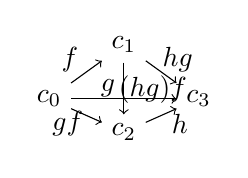
\begin{tikzpicture}[x=1.5em,y=1.5em]
  \node (c0) at (0,0.8) {$c_0$};
  \node (c1) at (1.8,2.1) {$c_1$};
  \node (c2) at (1.8,0) {$c_2$};
  \node (c3) at (3.6,0.8) {$c_3$};
  \draw[->] (c0) -- (c1);
  \node at (0.5,1.75) {$f$};
  \draw[->] (c1) -- (c3);
  \node at (3.1,1.75) {$hg$};
  \draw[->] (c0) -- (c3);
  \node at (2.5,1.02) {$(hg)f$};
  \draw[->] (c0) -- (c2);
  \node at (0.45,0.2) {$gf$};
  \draw[->] (c2) -- (c3);
  \node at (3.15,0.2) {$h$};
  \draw[->] (c1) -- (c2);
  \node at (1.42,1.05) {$g$};
\end{tikzpicture}
\end{center}
由于合成满足结合律，箭头 $(hg)f$ 同样是 $gf$ 接 $h$ 的复合，这就证得
顶点 $c_1$ 对面的 2-\trSimplex{}存在于 $C$ 中；再由 2-余骨架性，填充这一边界
球面的 3-\trSimplex{}也存在于 $C$ 中。\trHorn $\Lambda^2[3]\to C$ 的\trFiller{}可
类似地构造。
\end{proof}

\begin{definition}[1-\trSimplex{}上的\trHomotopyRelation]\label{def:homotopy-1-simplices}
\trSimplicialSet $X$ 中平行的 1-\trSimplex{} $f$ 与 $g$ 称为\textbf{\trHomotopy{}的}
（homotopic），若存在一个 2-\trSimplex{}，其边界取下列两种形状之一，
\footnote{记号「═」在图中表示一个退化单纯形或恒等箭头。}
\begin{rveq}\label{eq:homotopic-forms}
\mbox{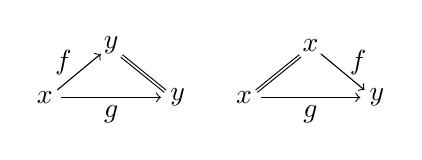
\begin{tikzpicture}[x=1.5em,y=1.5em]
  \node (x1) at (0,0) {$x$};
  \node (y1) at (1.6,1.25) {$y$};
  \node (y2) at (3.2,0) {$y$};
  \draw[->] (0.3,0.18) -- (1.35,1.05);
  \node at (0.45,0.85) {$f$};
  \draw[double] (1.85,1.0) -- (2.9,0.15);
  \draw[->] (0.4,0) -- (2.8,0);
  \node at (1.6,-0.4) {$g$};
  \node (x3) at (6.4,1.25) {$x$};
  \node (x4) at (4.8,0) {$x$};
  \node (y3) at (8.0,0) {$y$};
  \draw[double] (5.1,0.15) -- (6.15,1.0);
  \draw[->] (6.65,1.05) -- (7.7,0.18);
  \node at (7.55,0.85) {$f$};
  \draw[->] (5.2,0) -- (7.6,0);
  \node at (6.4,-0.4) {$g$};
\end{tikzpicture}}
\end{rveq}
或者 $f$ 与 $g$ 落在这一关系所生成的同一个\trEquivalence{}类里。
\end{definition}

在\trQuasiCategory{}中，由\eqref{eq:homotopic-forms}所展示的任一类型的 2-\trSimplex{}所
见证的关系都是\trEquivalence{}关系，而且这两种\trEquivalence{}关系重合。

\begin{lemma}[\trQuasiCategory{}中\trHomotopy{}的 1-\trSimplex]\label{lem:homotopic-quasi-category}
\trQuasiCategory{}中平行的 1-\trSimplex{} $f$ 与 $g$ 是\trHomotopy{}的，当且仅当存在一个
\eqref{eq:homotopic-forms}所示任一形状——\trEquivalence{}地，所有形状——的
2-\trSimplex{}。
\end{lemma}
\begin{proof}
见\cref{ex:homotopy-equivalence}。
\end{proof}

\begin{definition}[\trHomotopyCategory{}；\cite{bib44}~\S2.4]\label{def:homotopy-category}
经 1-截断，任何\trSimplicialSet $X$ 都带有底层的\textbf{\trReflexiveDirectedGraph}
（reflexive directed graph）：$X$ 的 0-\trSimplex{}定义对象，1-\trSimplex{}定义箭头：
\[
X_1\!
\begin{array}{@{}c@{}}
\xrightarrow{\;\cdot\delta^1\;}\\[-3pt]
\xleftarrow[\;\cdot\sigma^0\;]{}\\[-3pt]
\xrightarrow[\;\cdot\delta^0\;]{}
\end{array}
\!X_0,
\]
依约定，箭头 $f\in X_1$ 的来源是其第 0 个面 $f\cdot\delta^1$（顶点 1
对面的面），目标是其第 1 个面 $f\cdot\delta^0$（顶点 0 对面的面）。
这个\trReflexiveDirectedGraph{}上的\textbf{\trFreeCategory}（free category）以 $X_0$ 为对象集，
退化 1-\trSimplex{}充当恒等态射，而非恒等态射定义为非退化 1-\trSimplex{}的有限
有向路径。$X$ 的\textbf{\trHomotopyCategory}（homotopy category）$\mathrm{h}X$ 定义为：
底层\trReflexiveDirectedGraph{}上的\trFreeCategory{}对下述\trCongruence{}（congruence）\footnote{1-\trCategory{}的
平行箭头之间的二元关系 $\sim$ 称为\textbf{\trCongruence}，若它既是\trEquivalence{}关系又对
合成前与合成后封闭：若 $f\sim g$ 则 $hfk\sim hgk$。}取商所得者，
其中强加了由 2-单纯形见证的合成关系 $h=g\circ f$：
\begin{center}
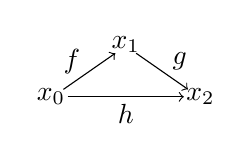
\begin{tikzpicture}[x=1.5em,y=1.5em]
  \node (x0) at (0,0) {$x_0$};
  \node (x1) at (1.8,1.25) {$x_1$};
  \node (x2) at (3.6,0) {$x_2$};
  \draw[->] (0.3,0.18) -- (1.55,1.05);
  \node at (0.5,0.85) {$f$};
  \draw[->] (2.05,1.05) -- (3.3,0.18);
  \node at (3.1,0.85) {$g$};
  \draw[->] (0.4,0) -- (3.2,0);
  \node at (1.8,-0.4) {$h$};
\end{tikzpicture}
\end{center}
这一关系特别地蕴含：\trHomotopy{}的 1-单纯形在\trHomotopyCategory{}中表示同一个箭头。
\end{definition}

1-\trCategory{}之\trNerve{}的\trHomotopyCategory\trIsomorphism{}于原来的\trCategory{}，因为\trNerve{}中的 2-\trSimplex{}见证了
底层\trReflexiveDirectedGraph{}的箭头所满足的全部合成关系。事实上，自然\trIsomorphism
$\mathrm{h}C\cong C$ 构成一个\trAdjunction{}的余单位（counit），
它把 $\mathcal{C}at$ 嵌入为 $s\mathcal{S}et$ 的反射子\trCategory
（reflective subcategory）。

\begin{proposition}\label{prop:nerve-left-adjoint}
\trNerve{}嵌入有左\trAdjunction{}，即把\trSimplicialSet{}送到其\trHomotopyCategory{}的\trFunctor{}：
\begin{center}
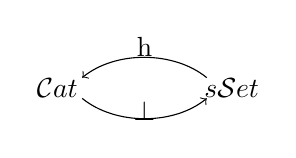
\begin{tikzpicture}[x=1.5em,y=1.5em]
  \node (cat) at (0,0) {$\mathcal{C}at$};
  \node (sset) at (4.2,0) {$s\mathcal{S}et$};
  \draw[->] (3.6,0.25) .. controls (2.8,0.9) and (1.4,0.9) .. (0.6,0.25);
  \node at (2.1,1.0) {$\mathrm{h}$};
  \draw[->] (0.6,-0.25) .. controls (1.4,-0.9) and (2.8,-0.9) .. (3.6,-0.25);
  \node at (2.1,-0.55) {$\perp$};
\end{tikzpicture}
\end{center}
\end{proposition}

\cref{prop:nerve-left-adjoint}的\trAdjunction{}对出于形式理由即可存在
（见\cref{ex:nerve-cosimplicial}），但直接的证明仍富有启发性。

\begin{proof}
对任何\trSimplicialSet $X$，都存在从 $X$ 到其\trHomotopyCategory{}之\trNerve $\mathrm{h}X$ 的自然
映射；由于\trNerve{}是\trTwoCoskeletal{}，只需定义 $\mathrm{sk}_2\,X\to\mathrm{h}X$，
而这由\cref{def:homotopy-category}的构造立即给出。注意：把\trHomotopyCategory\trFunctor
作用于商映射 $X\to\mathrm{h}X$ 后它变成\trIsomorphism{}，而且只要 $X$ 本是某个\trCategory{}的%
\trNerve{}，它就已经是\trIsomorphism{}。于是\trAdjunction{}性由引理 B.4.2 得出，%
也可直接验证三角形等式。
\end{proof}

\trQuasiCategory{}的\trHomotopyCategory{}容许一个简化了的描述。

\begin{lemma}[\trQuasiCategory{}的\trHomotopyCategory]\label{lem:homotopy-category-quasi-category}
若 $A$ 是\trQuasiCategory{}，则它的\textbf{\trHomotopyCategory} $\mathrm{h}A$ 具有：
\begin{itemize}
\item 对象：0-\trSimplex{}之集 $A_0$；
\item 箭头：1-\trSimplex{}之集 $A_1$ 的各\trHomotopy{}类；
\item 在 $a\in A_0$ 处的恒等箭头：由退化 1-\trSimplex{} $a\cdot\sigma^0\in A_1$
所表示；
\item $\mathrm{h}A$ 中的合成关系 $h=g\circ f$：对任意给定的 1-\trSimplex
$f$，$g$，$h\in A_1$ 所表示的箭头的\trHomotopy{}类而言，$h=g\circ f$ 成立当且仅当
存在一个边界为
\begin{center}
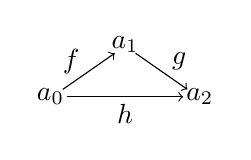
\begin{tikzpicture}[x=1.5em,y=1.5em]
  \node (a0) at (0,0) {$a_0$};
  \node (a1) at (1.8,1.25) {$a_1$};
  \node (a2) at (3.6,0) {$a_2$};
  \draw[->] (0.3,0.18) -- (1.55,1.05);
  \node at (0.5,0.85) {$f$};
  \draw[->] (2.05,1.05) -- (3.3,0.18);
  \node at (3.1,0.85) {$g$};
  \draw[->] (0.4,0) -- (3.2,0);
  \node at (1.8,-0.4) {$h$};
\end{tikzpicture}
\end{center}
的 2-\trSimplex{}。
\end{itemize}
\end{lemma}
\begin{proof}
见\cref{ex:homotopy-category-free-category}。
\end{proof}

\begin{definition}[\trQuasiCategory{}中的\trIsomorphism]\label{def:isomorphism-quasi-category}
\trQuasiCategory{}中的 1-\trSimplex{}是\textbf{\trIsomorphism}（isomorphism），\footnote{Joyal 称这些
映射为「\trIsomorphism」（isomorphism），而 Lurie 称之为「\trEquivalence」（equivalence）。
我们尽可能让\trInfinityCategory{}性概念与相应的 1-\trCategory{}性概念共用同一个称呼。}当且仅当
它在\trHomotopyCategory{}中表示一个\trIsomorphism{}。由\cref{lem:homotopy-category-quasi-category}，
这意味着：$f\colon a\to b$ 是\trIsomorphism{}，当且仅当存在 1-\trSimplex
$f^{-1}\colon b\to a$ 连同一对 2-\trSimplex
\begin{center}
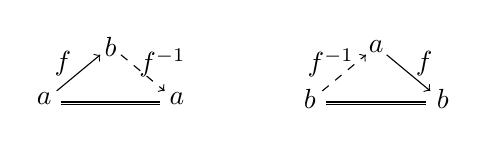
\begin{tikzpicture}[x=1.5em,y=1.5em]
  \node (a) at (0,0) {$a$};
  \node (b) at (1.6,1.25) {$b$};
  \node (a2) at (3.2,0) {$a$};
  \draw[->] (0.3,0.18) -- (1.35,1.05);
  \node at (0.45,0.85) {$f$};
  \draw[->,dashed] (1.85,1.05) -- (2.9,0.18);
  \node at (2.85,0.85) {$f^{-1}$};
  \draw[double] (0.4,-0.12) -- (2.8,-0.12);
  \node (b2) at (6.4,0) {$b$};
  \node (a3) at (8.0,1.25) {$a$};
  \node (b3) at (9.6,0) {$b$};
  \draw[->,dashed] (6.7,0.18) -- (7.75,1.05);
  \node at (6.9,0.85) {$f^{-1}$};
  \draw[->] (8.25,1.05) -- (9.3,0.18);
  \node at (9.15,0.85) {$f$};
  \draw[double] (6.8,-0.12) -- (9.2,-0.12);
\end{tikzpicture}
\end{center}
\end{definition}

\trQuasiCategory{}中\trIsomorphism{}的性质，最容易在一个密切相关的\trCategory{}中论证：那里的%
\trSimplicialSet{}带有额外的结构——在指定的 1-单纯形子集上做一个「标记」（marking）；
这些所谓的\textbf{\trMarkedSimplicialSet}（marked simplicial set）之间的
映射必须保持标记（见定义 D.1.1）。%
例如，每个\trQuasiCategory{}都有一个\emph{自然标记}（natural marking），其中带标记的
1-单纯形恰好是全部\trIsomorphism{}（见定义 D.4.5）。%
由于「\trQuasiCategory{}中是\trIsomorphism」这一性质由具有特定边界的 2-\trSimplex{}之存在所见证，
\trQuasiCategory{}之间的每个映射都保持\trIsomorphism{}，从而诱导出相应的自然带标记\trQuasiCategory{}之间的
映射。\trMarkedSimplicialSet{}很少出现在关于\trQuasiCategory{}中\trIsomorphism{}的某些组合引理的证明之外，
故细节留待附录 D。

现在来引出用标记技术证明的若干结果中的第一个。\trQuasiCategory $A$ 按定义沿一切
内\trHorn{}都有\trExtension{}。但当外\trHorn $\Lambda^0[2]\to A$ 或 $\Lambda^2[2]\to A$
的始边、终边（视情形而定）映成 $A$ 中的\trIsomorphism{}时，直觉上应当存在\trFiller

\begin{center}
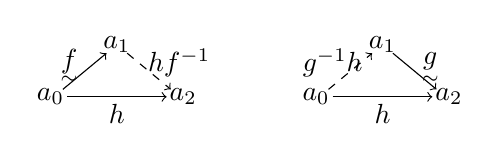
\begin{tikzpicture}[x=1.5em,y=1.5em]
  \node (a0) at (0,0) {$a_0$};
  \node (a1) at (1.6,1.25) {$a_1$};
  \node (a2) at (3.2,0) {$a_2$};
  \draw[->] (0.3,0.18) -- (1.35,1.05);
  \node at (0.45,0.85) {$f$};
  \node at (0.45,0.42) {$\scriptstyle\sim$};
  \draw[->,dashed] (1.85,1.05) -- (2.9,0.18);
  \node at (3.1,0.82) {$hf^{-1}$};
  \draw[->] (0.4,0) -- (2.8,0);
  \node at (1.6,-0.4) {$h$};
  \node (b0) at (6.4,0) {$a_0$};
  \node (b1) at (8.0,1.25) {$a_1$};
  \node (b2) at (9.6,0) {$a_2$};
  \draw[->,dashed] (6.7,0.18) -- (7.75,1.05);
  \node at (6.8,0.82) {$g^{-1}h$};
  \draw[->] (8.25,1.05) -- (9.3,0.18);
  \node at (9.15,0.85) {$g$};
  \node at (9.15,0.42) {$\scriptstyle\sim$};
  \draw[->] (6.8,0) -- (9.2,0);
  \node at (8.0,-0.4) {$h$};
\end{tikzpicture}
\end{center}
高维的「特殊外\trHorn」的表现类似：

\begin{proposition}[特殊外\trHorn{}填充]\label{prop:special-outer-horn-filling}
任何\trQuasiCategory $A$ 对下面这些外\trHorn
\begin{center}
\begin{tikzpicture}[x=1.4em,y=1.4em]
  \node (tl) at (0,1.2) {$\Lambda^0[n]$};
  \node (tr) at (3.0,1.2) {$A$};
  \node (bl) at (0,0) {$\Delta[n]$};
  \draw[->] (tl) -- (tr);
  \node at (1.5,1.52) {$g$};
  \draw[->] (0,0.85) -- (0,0.28);
  \draw (0,0.85) arc[start angle=180,end angle=0,radius=0.15];
  \draw[->,dashed] (0.5,0.22) -- (2.7,1.05);
  \node (tl2) at (6.6,1.2) {$\Lambda^n[n]$};
  \node (tr2) at (9.6,1.2) {$A$};
  \node (bl2) at (6.6,0) {$\Delta[n]$};
  \draw[->] (tl2) -- (tr2);
  \node at (8.1,1.52) {$h$};
  \draw[->] (6.6,0.85) -- (6.6,0.28);
  \draw (6.6,0.85) arc[start angle=180,end angle=0,radius=0.15];
  \draw[->,dashed] (7.1,0.22) -- (9.3,1.05);
  \node at (11.8,0.6) {对 $n\ge 1$};
\end{tikzpicture}
\end{center}
都有\trFiller{}，只要其中边 $g|_{\langle\,0,1\,\rangle}$ 与 $h|_{\langle\,n-1,n\,\rangle}$ 是\trIsomorphism{}。
\footnote{当 $n=1$ 时，对\trHorn{}无须任何条件；退化 1-\trSimplex{}给出所需的\trLifting{}。}
\end{proposition}

\cref{prop:special-outer-horn-filling}的证明需要归功于 Joyal 的巧妙组合
技术，我们将其推延到命题 D.4.6。%
这里且先坐享其众多推论。立即可得：

\begin{corollary}\label{cor:kan-groupoid}
\trQuasiCategory{}是\trKanComplex{}，当且仅当它的\trHomotopyCategory{}是\trGroupoid{}（groupoid）。
\end{corollary}
\begin{proof}
若\trQuasiCategory{}的\trHomotopyCategory{}是\trGroupoid{}，则它的全部 1-\trSimplex{}都是\trIsomorphism{}，于是
\cref{prop:special-outer-horn-filling}蕴含一切内、外\trHorn{}都有\trFiller{}，
因此该\trQuasiCategory{}是\trKanComplex{}。反之，在\trKanComplex{}中一切外\trHorn{}都可填充；
特别地，\cref{def:isomorphism-quasi-category}中所示的那些\trHorn{}的\trFiller
可用来为任何 1-\trSimplex{}构造左逆与右逆，再由
\cref{lem:homotopy-category-quasi-category}把它们矫正成单一的双侧逆。
\end{proof}

\trQuasiCategory $A$ 含有一个典范的\textbf{\trMaximalSubKanComplex}（maximal sub Kan
complex）$A^{\simeq}$，即由那些作为\trIsomorphism{}的 1-\trSimplex{}张成的单纯子集。
正如\trQuasiCategory $A$ 中的箭头由\trSimplicialSet{}映射 $\qcTwo\to A$ 表示——其定义域是
\emph{\trFreeLivingArrow}（free-living arrow）的\trNerve——\trQuasiCategory{}中的\trIsomorphism{}也可以由图形
$\qcInt\to A$ 表示，其定义域称作\textbf{\trHomotopyCoherentIsomorphism}（homotopy
coherent isomorphism），即\emph{\trFreeLivingIsomorphism}（free-living isomorphism）的\trNerve{}：

\begin{corollary}\label{cor:hc-isomorphism}
\trQuasiCategory $A$ 中的箭头 $f$ 是\trIsomorphism{}，当且仅当它可\trExtension{}成一个\trHomotopyCoherentIsomorphism
\begin{center}
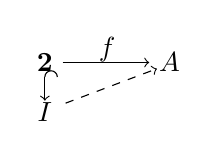
\begin{tikzpicture}[x=1.5em,y=1.5em]
  \node (tl) at (0,1.2) {$\qcTwo$};
  \node (tr) at (3.0,1.2) {$A$};
  \node (bl) at (0,0) {$\qcInt$};
  \draw[->] (tl) -- (tr);
  \node at (1.5,1.52) {$f$};
  \draw[->] (0,0.85) -- (0,0.28);
  \draw (0,0.85) arc[start angle=180,end angle=0,radius=0.15];
  \draw[->,dashed] (0.5,0.22) -- (2.7,1.05);
\end{tikzpicture}
\end{center}
\end{corollary}
\begin{proof}
若 $f$ 是\trIsomorphism{}，则映射 $f\colon\qcTwo\to A$ 落入含于 $A$ 中的极大子%
\trKanComplex{}：
\begin{center}
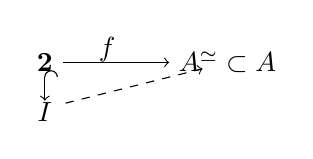
\begin{tikzpicture}[x=1.5em,y=1.5em]
  \node (tl) at (0,1.2) {$\qcTwo$};
  \node (tr) at (4.4,1.2) {$A^{\simeq}\subset A$};
  \node (bl) at (0,0) {$\qcInt$};
  \draw[->] (tl) -- (tr);
  \node at (1.5,1.52) {$f$};
  \draw[->] (0,0.85) -- (0,0.28);
  \draw (0,0.85) arc[start angle=180,end angle=0,radius=0.15];
  \draw[->,dashed] (0.5,0.22) -- (3.8,1.05);
\end{tikzpicture}
\end{center}
由\cref{ex:free-living-isomorphism}，包含 $\qcTwo\hookrightarrow\qcInt$
可以表示成外\trHorn{}包含之\trPushout{}（pushout）的序列复合。由于 $A^{\simeq}$ 是%
\trKanComplex{}，这表明所需的\trExtension{}存在，而且实际上落入 $A^{\simeq}\subset A$。
\end{proof}

\trSimplicialSet{}的\trCategory{}如同任何预层\trCategory{}一样是\trCartesianClosed{}。
由\trYonedaLemma{}与定义性\trAdjunction{}，指数 $Y^X$ 中的 $n$-\trSimplex{}对应于%
\trSimplicialSet{}映射 $X\times\Delta[n]\to Y$，它的面与退化通过在\trSimplex{}变量中预合成
来计算。我们的下一个目标是证明：\trQuasiCategory{}构成\trSimplicialSet{}这个\trSimpliciallyEnrichedCategory{}中的一个
\textbf{\trExponentialIdeal}（exponential ideal）：若 $X$ 是\trSimplicialSet{}而 $A$ 是\trQuasiCategory{}，
则 $A^X$ 是\trQuasiCategory{}。我们将把它当作该结果之「相对」版本的推论导出，后者涉及
一类叫做\trIsofibration{}的映射，现在就来引入。

\begin{definition}[\trIsofibration]\label{def:isofibration}
\trQuasiCategory{}之间的\trSimplicialSet{}映射 $f\colon A\to B$ 是一个\textbf{\trIsofibration}
（isofibration），若它对内\trHorn{}包含——如左下图所示——以及任一顶点向自由%
\trIsomorphism $\qcInt$ 的包含都能\trLifting{}：
\begin{center}
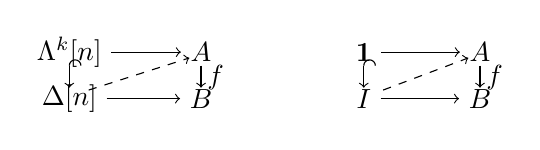
\begin{tikzpicture}[x=1.4em,y=1.4em]
  \node (tl) at (0,1.2) {$\Lambda^k[n]$};
  \node (tr) at (3.4,1.2) {$A$};
  \node (bl) at (0,0) {$\Delta[n]$};
  \node (br) at (3.4,0) {$B$};
  \draw[->] (tl) -- (tr);
  \draw[->] (0,0.85) -- (0,0.28);
  \draw (0,0.85) arc[start angle=180,end angle=0,radius=0.15];
  \draw[->,dashed] (0.5,0.22) -- (3.1,1.05);
  \draw[->] (3.4,0.85) -- (3.4,0.28);
  \node at (3.78,0.55) {$f$};
  \draw[->] (bl) -- (br);
  \node (tl2) at (7.6,1.2) {$\qcOne$};
  \node (tr2) at (10.6,1.2) {$A$};
  \node (bl2) at (7.6,0) {$\qcInt$};
  \node (br2) at (10.6,0) {$B$};
  \draw[->] (tl2) -- (tr2);
  \draw[->] (7.6,0.85) -- (7.6,0.28);
  \draw (7.6,0.85) arc[start angle=180,end angle=0,radius=0.15];
  \draw[->,dashed] (8.1,0.22) -- (10.3,1.05);
  \draw[->] (10.6,0.85) -- (10.6,0.28);
  \node at (10.98,0.55) {$f$};
  \draw[->] (bl2) -- (br2);
\end{tikzpicture}
\end{center}
为了在记号上区分\trIsofibration{}，我们把它们画成带两个头的箭头
「$\twoheadrightarrow$」。
\end{definition}

命题 1.1.14 被其相对化类比所吸收，后者证为定理 D.5.1：%

\begin{proposition}[特殊外\trHorn\trLifting]\label{prop:special-outer-horn-lifting}
\trQuasiCategory{}之间的任何\trIsofibration $f\colon A\twoheadrightarrow B$ 对下面这些
外\trHorn
\begin{center}
\begin{tikzpicture}[x=1.4em,y=1.4em]
  \node (tl) at (0,1.2) {$\Lambda^0[n]$};
  \node (tr) at (3.4,1.2) {$A$};
  \node (bl) at (0,0) {$\Delta[n]$};
  \node (br) at (3.4,0) {$B$};
  \draw[->] (tl) -- (tr);
  \node at (1.5,1.52) {$g$};
  \draw[->] (0,0.85) -- (0,0.28);
  \draw (0,0.85) arc[start angle=180,end angle=0,radius=0.15];
  \draw[->,dashed] (0.5,0.22) -- (3.1,1.05);
  \draw[->] (3.4,0.85) -- (3.4,0.28);
  \node at (3.78,0.55) {$f$};
  \draw[->] (bl) -- (br);
  \node at (1.7,-0.38) {$k$};
  \node (tl2) at (7.6,1.2) {$\Lambda^n[n]$};
  \node (tr2) at (11.0,1.2) {$A$};
  \node (bl2) at (7.6,0) {$\Delta[n]$};
  \node (br2) at (11.0,0) {$B$};
  \draw[->] (tl2) -- (tr2);
  \node at (9.3,1.52) {$h$};
  \draw[->] (7.6,0.85) -- (7.6,0.28);
  \draw (7.6,0.85) arc[start angle=180,end angle=0,radius=0.15];
  \draw[->,dashed] (8.1,0.22) -- (10.7,1.05);
  \draw[->] (11.0,0.85) -- (11.0,0.28);
  \node at (11.38,0.55) {$f$};
  \draw[->] (bl2) -- (br2);
  \node at (9.3,-0.38) {$\ell$};
  \node at (13.4,0.6) {对 $n\ge 1$};
\end{tikzpicture}
\end{center}
都有\trLifting{}，只要其中边 $g|_{\langle\,0,1\,\rangle}$、$h|_{\langle\,n-1,n\,\rangle}$、$k|_{\langle\,0,1\,\rangle}$ 与
$\ell|_{\langle\,n-1,n\,\rangle}$ 都是\trIsomorphism{}。
\end{proposition}

\begin{observation}\label{obs:isofibration-basics}
\begin{enumerate}[label=(\roman*)]
\item 对任何\trSimplicialSet $X$，以\trTerminal{}\trSimplicialSet 1 为陪域的唯一映射 $X\to 1$
是\trIsofibration{}，当且仅当 $X$ 是\trQuasiCategory{}。
\item 任何由右提升性质（right lifting property）刻画的映射类——例如\trIsofibration{}——
都自动对合成、乘积、\trPullback{}（pullback）、收缩（retract）以及塔的
（逆）\trLimit{}封闭（见引理 C.2.3）。%
\item 把 (i) 与 (ii) 结合起来：若 $A\twoheadrightarrow B$ 是\trIsofibration{}，而 $B$ 是%
\trQuasiCategory{}，则 $A$ 也是。
\item \trIsofibration{}推广了那个同名的范畴论概念。\trCategory{}之间任何%
\trFunctor{} $f\colon A\to B$ 的\trNerve{}定义了一个对内\trHorn{}包含可\trLifting{}的\trSimplicialSet
映射。这个映射定义\trIsofibration{}，当且仅当：对 $B$ 中的任何\trIsomorphism{}以及 $A$ 中%
\trLifting{}其定义域或陪域的指定对象，$A$ 中总存在具有该定义域或陪域、且\trLifting{}该%
\trIsomorphism{}的\trIsomorphism{}。
\end{enumerate}
\end{observation}

难以建立得多的是\trIsofibration{}在「Leibniz\footnote{这个名字暗指微分学中的
Leibniz 法则，更确切地，暗指把引理 D.3.1 的\trLeibnizProduct{}的定义域等同于
棱柱（prism）的边界（见定义 C.2.8 与注 D.3.2）。}%
指数」（Leibniz exponential）构造下的稳定性，如图
\eqref{eq:leibniz-exponential}所示。这将由命题 D.5.2 证明。

\begin{proposition}\label{prop:leibniz-exponential}
若 $i\colon X\hookrightarrow Y$ 是\trMonomorphism{}，而
$f\colon A\twoheadrightarrow B$ 是\trIsofibration{}，那么诱导的 Leibniz 指数
映射 $i\widehat{\pitchfork}f$
\begin{rveq}\label{eq:leibniz-exponential}
\mbox{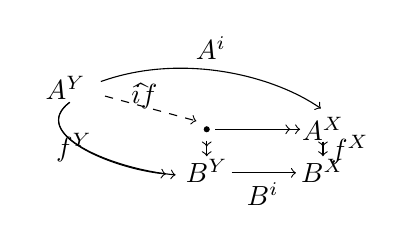
\begin{tikzpicture}[x=1.5em,y=1.5em]
  \node (AY) at (0,2.0) {$A^Y$};
  \fill (3.4,1.0) circle (1.1pt);
  \node (AX) at (6.2,1.0) {$A^X$};
  \node (BY) at (3.4,0) {$B^Y$};
  \node (BX) at (6.2,0) {$B^X$};
  \draw[->] (0.85,2.15) .. controls (2.8,2.85) and (5.0,2.3) .. (6.15,1.5);
  \node at (3.5,2.95) {$A^i$};
  \draw[->] (0.1,1.65) .. controls (-0.9,0.9) and (1.1,0.05) .. (2.65,-0.1);
  \draw[->,shorten >=0.35em] (0.1,1.65) .. controls (-0.9,0.9) and (1.1,0.05) .. (2.65,-0.1);
  \node at (0.2,0.55) {$f^Y$};
  \draw[->,dashed] (0.95,1.8) -- (3.15,1.2);
  \node at (1.9,1.8) {$i\widehat{\pitchfork}f$};
  \draw[->] (3.6,1.0) -- (5.65,1.0);
  \draw[->,shorten >=0.35em] (3.6,1.0) -- (5.65,1.0);
  \draw[->] (3.4,0.72) -- (3.4,0.35);
  \draw[->,shorten >=0.35em] (3.4,0.72) -- (3.4,0.35);
  \draw[->] (6.2,0.7) -- (6.2,0.35);
  \draw[->,shorten >=0.35em] (6.2,0.7) -- (6.2,0.35);
  \node at (6.85,0.5) {$f^X$};
  \draw[->] (4.0,-0.05) -- (5.55,-0.05);
  \node at (4.75,-0.55) {$B^i$};
  \node at (3.85,0.6) {$\lrcorner$};
\end{tikzpicture}}
\end{rveq}
仍是\trIsofibration{}。\footnote{这一结果的退化情形——取 $X=\varnothing$ 或
$B=1$——蕴含图中其余六个映射也都是\trIsofibration
（见\cref{ex:leibniz-specialization}）。}
\end{proposition}

\begin{corollary}\label{cor:exponential-ideal}
若 $X$ 是\trSimplicialSet{}而 $A$ 是\trQuasiCategory{}，则 $A^X$ 是\trQuasiCategory{}。此外，$A^X$ 中的
1-\trSimplex{}是\trIsomorphism{}，当且仅当它在 $X$ 的每个顶点处的分量都是 $A$ 中的\trIsomorphism{}。
\end{corollary}
\begin{proof}
第一句话是\cref{prop:leibniz-exponential}的特例
（见\cref{ex:leibniz-specialization}）；第二句话的证明类似，用带标记%
\trSimplicialSet{}来论证（见推论 D.4.19）。%
\end{proof}

\begin{definition}[\trQuasiCategory{}间的\trEquivalence]\label{def:equivalences-quasi-categories}
\trQuasiCategory{}之间的映射 $f\colon A\to B$ 是一个\textbf{\trEquivalence}
（equivalence），若它能\trExtension{}成一份以\trFreeLivingIsomorphism $\qcInt$ 充当区间
（interval）的「\trHomotopy\trEquivalence」数据；也就是说，若存在映射 $g\colon B\to A$，
\begin{center}
\begin{tikzpicture}[x=1.5em,y=1.5em]
  \node (Al) at (0,1.0) {$A$};
  \node (Ac) at (2.4,1.0) {$A^{\qcInt}$};
  \node (At) at (4.6,2.4) {$A$};
  \node (Ab) at (4.6,-0.4) {$A$};
  \draw[->] (0.4,1.0) -- (1.6,1.0);
  \node at (1.0,1.3) {$\alpha$};
  \draw[->] (2.7,1.3) -- (4.25,2.2);
  \node at (3.85,2.0) {$\mathrm{ev}_0$};
  \draw[->] (2.7,0.7) -- (4.25,-0.2);
  \node at (3.85,-0.1) {$\mathrm{ev}_1$};
  \draw[double] (0.35,1.4) -- (4.1,2.45);
  \draw[->] (0.4,0.6) -- (4.2,-0.28);
  \node at (1.7,0.02) {$gf$};
  \node at (7.4,1.0) {及};
  \node (Bl) at (10.0,1.0) {$B$};
  \node (Bc) at (12.4,1.0) {$B^{\qcInt}$};
  \node (Bt) at (14.6,2.4) {$B$};
  \node (Bb) at (14.6,-0.4) {$B$};
  \draw[->] (10.35,1.35) -- (14.1,2.45);
  \node at (11.3,2.15) {$fg$};
  \draw[->] (10.4,1.0) -- (11.6,1.0);
  \node at (11.0,1.3) {$\beta$};
  \draw[->] (12.7,1.3) -- (14.25,2.2);
  \node at (13.85,2.0) {$\mathrm{ev}_0$};
  \draw[->] (12.7,0.7) -- (14.25,-0.2);
  \node at (13.85,-0.1) {$\mathrm{ev}_1$};
  \draw[double] (10.35,0.6) -- (14.1,-0.35);
\end{tikzpicture}
\end{center}
我们写「$\qcEquiv$」来装饰\trEquivalence{}，并以 $A\simeq B$ 表示存在\trEquivalence
$A\qcEquiv B$。
\end{definition}

\begin{remark}\label{rem:hf-equivalence}
若 $f\colon A\to B$ 是\trQuasiCategory{}之间的\trEquivalence{}，则\trFunctor
$\mathrm{h}f\colon\mathrm{h}A\to\mathrm{h}B$ 是\trCategory{}的\trEquivalence{}；上面展示的
数据定义了\trEquivalence{}逆 $\mathrm{h}g\colon\mathrm{h}B\to\mathrm{h}A$ 以及由
复合\trFunctor\footnote{注意 $\mathrm{h}(A^{\qcInt})$ 与
$(\mathrm{h}A)^{\qcInt}$ 一般并不\trIsomorphism{}。后者中的对象是 $A$ 中\trIsomorphism{}的%
\trHomotopy{}类；前者中的对象则是\trHomotopyCoherentIsomorphism——由 $A$ 中一个指定的 1-单纯形、
一个指定的逆 1-单纯形，连同由 $\qcInt$ 的非退化单纯形标引的
相干性数据的无穷之塔给出。}编码而成的自然\trIsomorphism{}：
\[
\mathrm{h}A\xrightarrow{\;\mathrm{h}\alpha\;}\mathrm{h}(A^{\qcInt})
\longrightarrow(\mathrm{h}A)^{\qcInt}
\qquad\qquad
\mathrm{h}B\xrightarrow{\;\mathrm{h}\beta\;}\mathrm{h}(B^{\qcInt})
\longrightarrow(\mathrm{h}B)^{\qcInt}
\]
\end{remark}

\begin{definition}\label{def:trivial-fibration}
\trSimplicialSet{}之间的映射 $f\colon X\to Y$ 是一个\textbf{\trTrivialFibration}
（trivial fibration），若它对一切单纯形的边界包含都能\trLifting{}：
\begin{rveq}\label{eq:trivial-fibration}
\mbox{\begin{tikzpicture}[x=1.5em,y=1.5em]
  \node (tl) at (0,1.2) {$\partial\Delta[n]$};
  \node (tr) at (3.4,1.2) {$X$};
  \node (bl) at (0,0) {$\Delta[n]$};
  \node (br) at (3.4,0) {$Y$};
  \draw[->] (tl) -- (tr);
  \draw[->] (0,0.85) -- (0,0.28);
  \draw (0,0.85) arc[start angle=180,end angle=0,radius=0.15];
  \draw[->,dashed] (0.5,0.22) -- (3.1,1.05);
  \draw[->] (3.4,0.85) -- (3.4,0.28);
  \draw[->,shorten >=0.35em] (3.4,0.85) -- (3.4,0.28);
  \node at (3.0,0.55) {$\wr$};
  \node at (3.82,0.55) {$f$};
  \draw[->] (bl) -- (br);
  \node at (8.0,0.6) {对 $n\ge 0$};
\end{tikzpicture}}
\end{rveq}
我们写「$\qcTFib$」来装饰\trTrivialFibration{}。
\end{definition}

\begin{remark}\label{rem:trivial-fibration-notation}
\trSimplex{}边界包含 $\partial\Delta[n]\hookrightarrow\Delta[n]$
「\trCell{}式地生成」（cellularly generate）\trSimplicialSet{}的\trMonomorphism
（见定义 C.2.4 与引理 C.5.9）。%
于是引理 C.2.3 的对偶命题蕴含：\trTrivialFibration{}对\trSimplicialSet{}之间的任何\trMonomorphism{}都能%
\trLifting{}。特别地，由此可知任何\trTrivialFibration $X\qcTFib Y$ 都是\trSplitEpimorphism
（split epimorphism）。

记号「$\qcTFib$」是有暗示意味的：\trQuasiCategory{}之间的\trTrivialFibration{}恰好就是那些既是%
\trIsofibration{}又是\trEquivalence{}的映射。这一点可以用单纯\trHomotopy{}论中一个相当标准、只是
颇为技术性的论证来证明，见命题 D.5.6。%
\end{remark}

\begin{proposition}\label{prop:trivial-fibration-characterization}
对\trQuasiCategory{}之间的映射 $f\colon A\to B$，下列诸条件\trEquivalence{}：
\begin{enumerate}[label=(\roman*)]
\item $f$ 是\trTrivialFibration{}；
\item $f$ 既是\trIsofibration{}又是\trEquivalence{}；
\item $f$ 是\textbf{\trSplitFiberHomotopyEquivalence}（split fiber homotopy
equivalence）：一个\trIsofibration{}，它容许一个\trSection{}（section）$s$，这个截面
经由从 $\mathrm{id}_A$ 到 $sf$ 的\trHomotopy $\alpha$ 而成为\trEquivalence{}逆，且该\trHomotopy{}与
$f$ 复合后给出从 $f$ 到 $f$ 的常值\trHomotopy{}。
\begin{center}
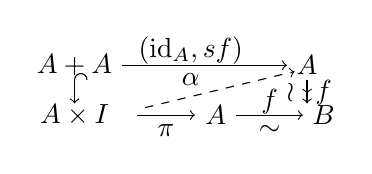
\begin{tikzpicture}[x=1.5em,y=1.5em]
  \node (tl) at (0,1.2) {$A+A$};
  \node (tr) at (5.6,1.2) {$A$};
  \node (bl) at (0,0) {$A\times\qcInt$};
  \node (bm) at (3.4,0) {$A$};
  \node (br) at (6.0,0) {$B$};
  \draw[->] (tl) -- (tr);
  \node at (2.8,1.55) {$(\mathrm{id}_A,sf)$};
  \draw[->] (0,0.85) -- (0,0.28);
  \draw (0,0.85) arc[start angle=180,end angle=0,radius=0.15];
  \draw[->,dashed] (1.7,0.18) -- (5.3,1.05);
  \node at (2.8,0.85) {$\alpha$};
  \draw[->] (5.6,0.85) -- (5.6,0.28);
  \draw[->,shorten >=0.35em] (5.6,0.85) -- (5.6,0.28);
  \node at (5.2,0.55) {$\wr$};
  \node at (6.0,0.55) {$f$};
  \draw[->] (1.5,0) -- (2.9,0);
  \node at (2.2,-0.38) {$\pi$};
  \draw[->] (3.9,0) -- (5.5,0);
  \node at (4.7,0.32) {$f$};
  \node at (4.7,-0.38) {$\sim$};
\end{tikzpicture}
\end{center}
\end{enumerate}
\end{proposition}

作为由右提升性质刻画的类，\trTrivialFibration{}还对合成、乘积、\trPullback{}与塔的%
\trLimit{}封闭，并且包含全部\trIsomorphism{}。这些映射在 Leibniz 指数化下的稳定性，
与\cref{prop:leibniz-exponential}一起在命题 D.5.2 中得到证明。

\begin{proposition}\label{prop:leibniz-exponential-trivial}
若 $i\colon X\hookrightarrow Y$ 是\trMonomorphism{}而 $f\colon A\twoheadrightarrow B$
是\trIsofibration{}，那么当 $f$ 是\trTrivialFibration{}，或者 $i$ 属于由内\trHorn{}包含与映射
$\qcOne\hookrightarrow\qcInt$ \trCell{}式生成的类时，诱导的 Leibniz 指数映射
\[
A^Y\xrightarrow{\;i\widehat{\pitchfork}f\;}B^Y\times_{B^X}A^X
\]
是\trTrivialFibration{}。
\end{proposition}

为展示这些 Leibniz 稳定性结果的效用，我们给出\trKanComplex{}的一个「内蕴的」
或「综合的」刻画。

\begin{lemma}\label{lem:kan-internal}
\trQuasiCategory $A$ 是\trKanComplex{}，当且仅当由包含 $\qcTwo\hookrightarrow\qcInt$
诱导的映射 $A^{\qcInt}\qcTFib A^{\qcTwo}$ 是\trTrivialFibration{}。
\end{lemma}

注意\cref{prop:leibniz-exponential}蕴含
$A^{\qcInt}\twoheadrightarrow A^{\qcTwo}$ 是\trIsofibration{}。
\begin{proof}
刻画\trTrivialFibration{}的那个提升性质可以转置成另一个提升性质，如右下图所示：
\begin{center}
\begin{tikzpicture}[x=1.4em,y=1.4em]
  \node (tl) at (0,1.2) {$\partial\Delta[n]$};
  \node (tr) at (3.4,1.2) {$A^{\qcInt}$};
  \node (bl) at (0,0) {$\Delta[n]$};
  \node (br) at (3.4,0) {$A^{\qcTwo}$};
  \draw[->] (tl) -- (tr);
  \draw[->] (0,0.85) -- (0,0.28);
  \draw (0,0.85) arc[start angle=180,end angle=0,radius=0.15];
  \draw[->,dashed] (0.5,0.22) -- (3.1,1.05);
  \draw[->] (3.4,0.85) -- (3.4,0.28);
  \draw[->] (bl) -- (br);
  \node at (6.6,0.6) {$\leftrightsquigarrow$};
  \node (TL) at (11.2,1.2)
    {$\partial\Delta[n]\times\qcInt\;\underset{\partial\Delta[n]\times\qcTwo}{\cup}\;\Delta[n]\times\qcTwo$};
  \node (TR) at (18.6,1.2) {$A$};
  \node (BL) at (11.2,0) {$\Delta[n]\times\qcInt$};
  \draw[->] (TL) -- (TR);
  \draw[->] (11.2,0.85) -- (11.2,0.28);
  \draw (11.2,0.85) arc[start angle=180,end angle=0,radius=0.15];
  \draw[->,dashed] (11.8,0.15) -- (18.3,1.05);
\end{tikzpicture}
\end{center}
它断言：$A$ 沿这样一些映射有\trExtension——它们由\trSimplex{}边界包含
$\partial\Delta[n]\hookrightarrow\Delta[n]$ 与包含
$\qcTwo\hookrightarrow\qcInt$ 作 \emph{\trLeibnizProduct}（Leibniz product，
又称\trPushout{}积（pushout product））而得。由\cref{ex:free-living-isomorphism}(ii)，
包含 $\qcTwo\hookrightarrow\qcInt$ 是左外\trHorn{}包含的\trPushout{}的序列复合。
由推论 D.3.11——它是通往\cref{prop:leibniz-exponential}与
\cref{prop:leibniz-exponential-trivial}之证明途中的关键一步——\trLeibnizProduct%
也是左外\trHorn{}包含与内\trHorn{}包含的\trPushout{}的序列复合。
若 $A$ 是\trKanComplex{}，则右上图所示的\trExtension{}存在，经转置便知
$A^{\qcInt}\qcTFib A^{\qcTwo}$ 是\trTrivialFibration{}。

反之，若 $A^{\qcInt}\qcTFib A^{\qcTwo}$ 是\trTrivialFibration{}，那么它特别地在
顶点上是满射。于是 $A$ 中的每个箭头都是\trIsomorphism{}，而\cref{cor:kan-groupoid}
告诉我们：$A$ 必定是\trKanComplex{}。
\end{proof}

\begin{digression}[Joyal \trModelStructure]\label{dig:joyal-model-structure}
\trSimplicialSet{}的\trCategory{}带有一个 Quillen 意义下（见定义 C.3.1）的
\textbf{\trModelStructure}（model structure），%
其\trFibrant{}对象（fibrant object）恰好是\trQuasiCategory{}，而且其中所有对象都是%
\trCofibrant{}的（cofibrant）。在\trFibrant{}对象之间，\trFibration{}、\trWeakEquivalence
（weak equivalence）与\trTrivialFibration{}恰是刚才引入的\trIsofibration{}、\trEquivalence{}与平凡%
\trFibration{}。\cref{prop:trivial-fibration-characterization}证明了\trTrivialFibration
是\trFibration{}与\trWeakEquivalence{}的交。\cref{prop:leibniz-exponential}与
\cref{prop:leibniz-exponential-trivial}则反映出：Joyal \trModelStructure{}是一个%
\trCartesianClosed\trModelCategory{}（cartesian closed model category），满足定义 C.3.10
的额外公理。%

我们不愿再进一步展开\trQuasiCategory{}上的 Joyal \trModelStructure{}，因为所需的全部特征都已
在此得到突出。这里列举的结果足以表明：\trQuasiCategory{}的\trCategory{}定义了一个%
\trInfinityCosmos——一个我们现在就要转入的概念。
\end{digression}

\subsection*{练习}

\begin{exercise}[\cite{bib103}~\S1.5]\label{ex:nerve-cosimplicial}
给定任意取值于任意\trCategory{} $\mathcal{E}$ 的\trCosimplicialObject
（cosimplicial object）$C\colon\Delta\to\mathcal{E}$，都有一个相伴的
\textbf{\trNerve{}函子} $N_C$，定义如下：
\[
\begin{array}{c}
\mathcal{E}\xrightarrow{\quad N_C\quad}s\mathcal{S}et\\[4pt]
E\longmapsto\mathrm{hom}(C^{-},E)
\end{array}
\qquad\qquad
\mbox{\begin{tikzpicture}[x=1.5em,y=1.5em]
  \node (D) at (2.4,2.1) {$\Delta$};
  \node (E) at (0,0) {$\mathcal{E}$};
  \node (S) at (4.8,0) {$s\mathcal{S}et$};
  \draw[->] (0.5,0.45) -- (1.95,1.8);
  \node at (0.65,1.35) {$C$};
  \draw[->] (2.85,1.8) -- (4.3,0.45);
  \node at (4.15,1.35) {よ};
  \draw[->] (4.25,0.2) .. controls (3.4,0.85) and (1.4,0.85) .. (0.55,0.2);
  \node at (2.4,0.98) {$\mathrm{lan}_{\text{よ}}C$};
  \node at (2.4,0.4) {$\perp$};
  \draw[->] (0.55,-0.2) .. controls (1.4,-0.75) and (3.4,-0.75) .. (4.25,-0.2);
  \node at (2.4,-1.05) {$N_C$};
\end{tikzpicture}}
\]
由构造，$N_CE$ 中的 $n$-\trSimplex{}对应 $\mathcal{E}$ 中的映射 $C^n\to E$。
证明：若 $\mathcal{E}$ \trCocomplete{}（cocomplete），则 $N_C$ 有左\trAdjunction{}，定义为%
\trFunctor{} $C$ 沿 \trYonedaEmbedding $\text{よ}\colon\Delta\hookrightarrow s\mathcal{S}et$ 的左\trKanExtension{}。这给出
\cref{prop:nerve-left-adjoint}的第二个证明。
\end{exercise}

\begin{exercise}[Boardman--Vogt；\cite{bib21}]\label{ex:homotopy-equivalence}
考虑\trQuasiCategory{}中以 $a$ 为\trInitial{}顶点、$b$ 为\trTerminal{}顶点的那些
1-单纯形之集。
\begin{enumerate}[label=(\roman*)]
\item 证明：由「$f\sim g$，当且仅当存在一个边界为
\tikz[baseline=-0.8ex]{\begin{scope}[x=1.3em,y=1.3em]
  \node (a) at (0,0) {$a$};
  \node (b) at (1.5,1.15) {$b$};
  \node (b2) at (3.0,0) {$b$};
  \draw[->] (0.28,0.16) -- (1.26,0.98);
  \node at (0.4,0.8) {$f$};
  \draw[double] (1.72,0.95) -- (2.72,0.14);
  \draw[->] (0.38,0) -- (2.62,0);
  \node at (1.5,-0.4) {$g$};
\end{scope}}
的 2-\trSimplex{}」所定义的关系是\trEquivalence{}关系。
\item 证明：由「$f\sim g$，当且仅当存在一个边界为
\tikz[baseline=-0.8ex]{\begin{scope}[x=1.3em,y=1.3em]
  \node (a) at (0,0) {$a$};
  \node (a2) at (1.5,1.15) {$a$};
  \node (b) at (3.0,0) {$b$};
  \draw[double] (0.28,0.14) -- (1.26,0.98);
  \draw[->] (1.74,0.98) -- (2.72,0.16);
  \node at (2.62,0.8) {$f$};
  \draw[->] (0.38,0) -- (2.62,0);
  \node at (1.5,-0.4) {$g$};
\end{scope}}
的 2-\trSimplex{}」所定义的关系是\trEquivalence{}关系。
\item 证明：(i) 与 (ii) 所定义的\trEquivalence{}关系是同一个。
\end{enumerate}
这就证明了\cref{lem:homotopic-quasi-category}。
\end{exercise}

\begin{exercise}\label{ex:homotopy-category-free-category}
考虑如下\trReflexiveDirectedGraph——它是一个\trQuasiCategory $A$ 的底层——上的\trFreeCategory{}：
\[
A_1\!
\begin{array}{@{}c@{}}
\xrightarrow{\;\cdot\delta^1\;}\\[-3pt]
\xleftarrow[\;\cdot\sigma^0\;]{}\\[-3pt]
\xrightarrow[\;\cdot\delta^0\;]{}
\end{array}
\!A_0,
\]
\begin{enumerate}[label=(\roman*)]
\item 考虑这样的二元关系：只要在 $A$ 的某个\trSimplex{}中，两列具有公共来源与
公共目标的可合成 1-\trSimplex{}给出从其\trInitial{}顶点到\trTerminal{}顶点的
两条路径，就把这两列等同起来。证明：这一关系对用 1-\trSimplex{}作合成前与
合成后是\trStable{}，并据此得出：它的\trTransitiveClosure{}是一个\textbf{\trCongruence}
（congruence）——即对合成前与合成后封闭的\trEquivalence{}关系。
\footnote{给定 1-\trCategory{}诸同态集上的一个\trCongruence{}关系，可以逐个同态集取商而
形成商范畴（见\cite{bib81}~\S II.8）。}
\item 考虑由强加合成关系 $h=g\circ f$ 所生成的\trCongruence{}关系——该关系由边界为
\tikz[baseline=-0.8ex]{\begin{scope}[x=1.3em,y=1.3em]
  \node (a0) at (0,0) {$a_0$};
  \node (a1) at (1.5,1.15) {$a_1$};
  \node (a2) at (3.0,0) {$a_2$};
  \draw[->] (0.28,0.16) -- (1.26,0.98);
  \node at (0.4,0.8) {$f$};
  \draw[->] (1.74,0.98) -- (2.72,0.16);
  \node at (2.62,0.8) {$g$};
  \draw[->] (0.38,0) -- (2.62,0);
  \node at (1.5,-0.4) {$h$};
\end{scope}}
的 2-\trSimplex{}见证——并证明它与 (i) 中所考虑的关系重合。
\item 在 (i) 与 (ii) 的\trCongruence{}关系中，证明：$A$ 中任何可合成 1-\trSimplex{}序列都\trEquivalence{}于单个
1-\trSimplex{}。据此得出：该\trFreeCategory{}对这个\trCongruence{}关系所取的商中的每个态射，都由
$A$ 中的一个 1-单纯形表示。
\item 证明：对 $A$ 中任意三个 1-\trSimplex{} $f$，$g$，$h$，在
\cref{def:homotopy-category}的\trHomotopyCategory $\mathrm{h}A$ 中 $h=g\circ f$
成立，当且仅当存在边界为
\tikz[baseline=-0.8ex]{\begin{scope}[x=1.3em,y=1.3em]
  \node (a0) at (0,0) {$a_0$};
  \node (a1) at (1.5,1.15) {$a_1$};
  \node (a2) at (3.0,0) {$a_2$};
  \draw[->] (0.28,0.16) -- (1.26,0.98);
  \node at (0.4,0.8) {$f$};
  \draw[->] (1.74,0.98) -- (2.72,0.16);
  \node at (2.62,0.8) {$g$};
  \draw[->] (0.38,0) -- (2.62,0);
  \node at (1.5,-0.4) {$h$};
\end{scope}}
的 2-\trSimplex{}。
\end{enumerate}
这就证明了\cref{lem:homotopy-category-quasi-category}。
\end{exercise}

\begin{exercise}\label{ex:unique-fillers}
证明：任何内\trHorn{}都有唯一\trFiller{}的\trQuasiCategory{}，\trIsomorphism{}于其\trHomotopyCategory{}的\trNerve{}。
\end{exercise}

\begin{exercise}\label{ex:free-living-isomorphism}
设 $\qcInt$ 是\trFreeLivingIsomorphism{}的\trNerve{}。
\begin{enumerate}[label=(\roman*)]
\item 证明：$\qcInt$ 在每个维数都恰有两个非退化\trSimplex{}。
\item 归纳地从 $\qcTwo$ 构筑出 $\qcInt$：把包含
$\qcTwo\hookrightarrow\qcInt$ 表示成左外\trHorn{}包含\footnote{按定义 1.2.25
所描述的对偶性，也可以换用右外\trHorn{}包含 $\Lambda^n[n]\hookrightarrow\Delta[n]$。}
$\Lambda^0[n]\hookrightarrow\Delta[n]$ 的\trPushout{}的序列复合，从 $n=2$ 开始
每维一个。\footnote{$\qcTwo\hookrightarrow\qcInt$ 的这一分解揭示了哪些
数据能\trHomotopy{}唯一地\trExtension{}成一个\trHomotopyCoherentIsomorphism{}。例如，\cref{def:isomorphism-quasi-category}
中的那些 1-\trSimplex{}与 2-\trSimplex{}，连同以它们为外表面而内表面皆退化的单个
3-\trSimplex{}。\trHomotopy{}类型论者把这份数据称作半\trAdjunction\trEquivalence{}（half adjoint
equivalence）\cite{bib125}~\S4.2。}
\end{enumerate}
\end{exercise}

\begin{exercise}\label{ex:relative-hc-isomorphism}
证明\cref{cor:hc-isomorphism}的相对版本：对\trQuasiCategory{}之间的任何\trIsofibration
$p\colon A\twoheadrightarrow B$ 与任何在 $A$ 中定义\trIsomorphism{}的
$f\colon\qcTwo\to A$，$B$ 中\trExtension{} $pf$ 的任何\trHomotopyCoherentIsomorphism{}都可\trLifting{}为 $A$
中\trExtension{} $f$ 的\trHomotopyCoherentIsomorphism{}：
\begin{center}
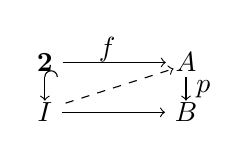
\begin{tikzpicture}[x=1.5em,y=1.5em]
  \node (tl) at (0,1.2) {$\qcTwo$};
  \node (tr) at (3.4,1.2) {$A$};
  \node (bl) at (0,0) {$\qcInt$};
  \node (br) at (3.4,0) {$B$};
  \draw[->] (tl) -- (tr);
  \node at (1.5,1.52) {$f$};
  \draw[->] (0,0.85) -- (0,0.28);
  \draw (0,0.85) arc[start angle=180,end angle=0,radius=0.15];
  \draw[->,dashed] (0.5,0.22) -- (3.1,1.05);
  \draw[->] (3.4,0.85) -- (3.4,0.28);
  \node at (3.82,0.55) {$p$};
  \draw[->] (bl) -- (br);
\end{tikzpicture}
\end{center}
\end{exercise}

\begin{exercise}\label{ex:leibniz-specialization}
将\cref{prop:leibniz-exponential}特化，以证明下列诸结论：
\begin{enumerate}[label=(\roman*)]
\item 若 $A$ 是\trQuasiCategory{}而 $X$ 是\trSimplicialSet{}，则 $A^X$ 是\trQuasiCategory{}。
\item 若 $A$ 是\trQuasiCategory{}而 $X\hookrightarrow Y$ 是\trMonomorphism{}，则
$A^Y\twoheadrightarrow A^X$ 是\trIsofibration{}。
\item 若 $A\twoheadrightarrow B$ 是\trIsofibration{}而 $X$ 是\trSimplicialSet{}，则
$A^X\twoheadrightarrow B^X$ 是\trIsofibration{}。
\end{enumerate}
\end{exercise}

\begin{exercise}\label{ex:equivalences-calculus}
预演引理 1.2.17：
\begin{enumerate}[label=(\roman*)]
\item 证明：\cref{def:equivalences-quasi-categories}所定义的\trEquivalence{}对收缩
封闭。
\item 证明：\cref{def:equivalences-quasi-categories}所定义的\trEquivalence{}满足%
\trTwoOfThreeProperty{}（2-of-3 property）。
\end{enumerate}
\end{exercise}

\begin{exercise}\label{ex:hf-surjective-equivalence}
证明：若 $f\colon X\qcTFib Y$ 是\trQuasiCategory{}之间的\trTrivialFibration{}，则\trFunctor
$\mathrm{h}f\colon\mathrm{h}X\qcEquiv\mathrm{h}Y$ 是\trCategory{}的\trSurjectiveEquivalence
（surjective equivalence）。
\end{exercise}
